% Golden Spiral can be approximated with Golden ratio or Fibonacci sequence.
% Golden Ratio: a+b/a = a/b

\documentclass{beamer}
\usepackage[utf8]{inputenc}
\usepackage[T1]{fontenc}
\usepackage{graphicx}

\usetheme{Cuerna}
\usecolortheme{default}
% default, bluesimplex, lettuce, brick

% slide (frames) numbering
\addtobeamertemplate{navigation symbols}{}{
    \usebeamerfont{footline}%
    \usebeamercolor[fg]{footline}%
    \hspace{1em}%
    \insertframenumber/\inserttotalframenumber
}

\title{TITLE}
\author{Shayan Amani}

\date{DATE 2019}
\institute{Department of Computer Science, University of New Hampshire}

\begin{document}

  \begin{frame}
    \titlepage
  \end{frame}
  
  
%%%%%% Slides begin

\begin{frame}
\frametitle{They have said...}

\Huge{``Our virtues and our failings are \textbf{inseparable}, like force and matter. When they separate, \textbf{man is no more}.''}

% \begin{rightflush}
% Nikola Tesla
% \end{rightflush}
\hfill \LARGE{\textit{Nikola Tesla}}

    
\end{frame}

\begin{frame}
    \frametitle{Who Am I?}
    
    I...
    \begin{itemize}
        \item finished my bachelor's in electrical engineering in 2015
        \item aspired to develop for my own ideas --at a certain point, I had 200k monthly active users on one of my applications--
        \item started my Ph.D. program at UNH in fall 2017
        \item have been through a journey to figure out what I want
        \item have been experimenting with quite a few areas
        \item ended up working with Prof. Marek Petrik on RL
    \end{itemize}
    
    \note{journey of discovering new things}
    \note{tiptoeing different waters}
\end{frame}

\begin{frame}
    \frametitle{What Have I Been Dealing With}
    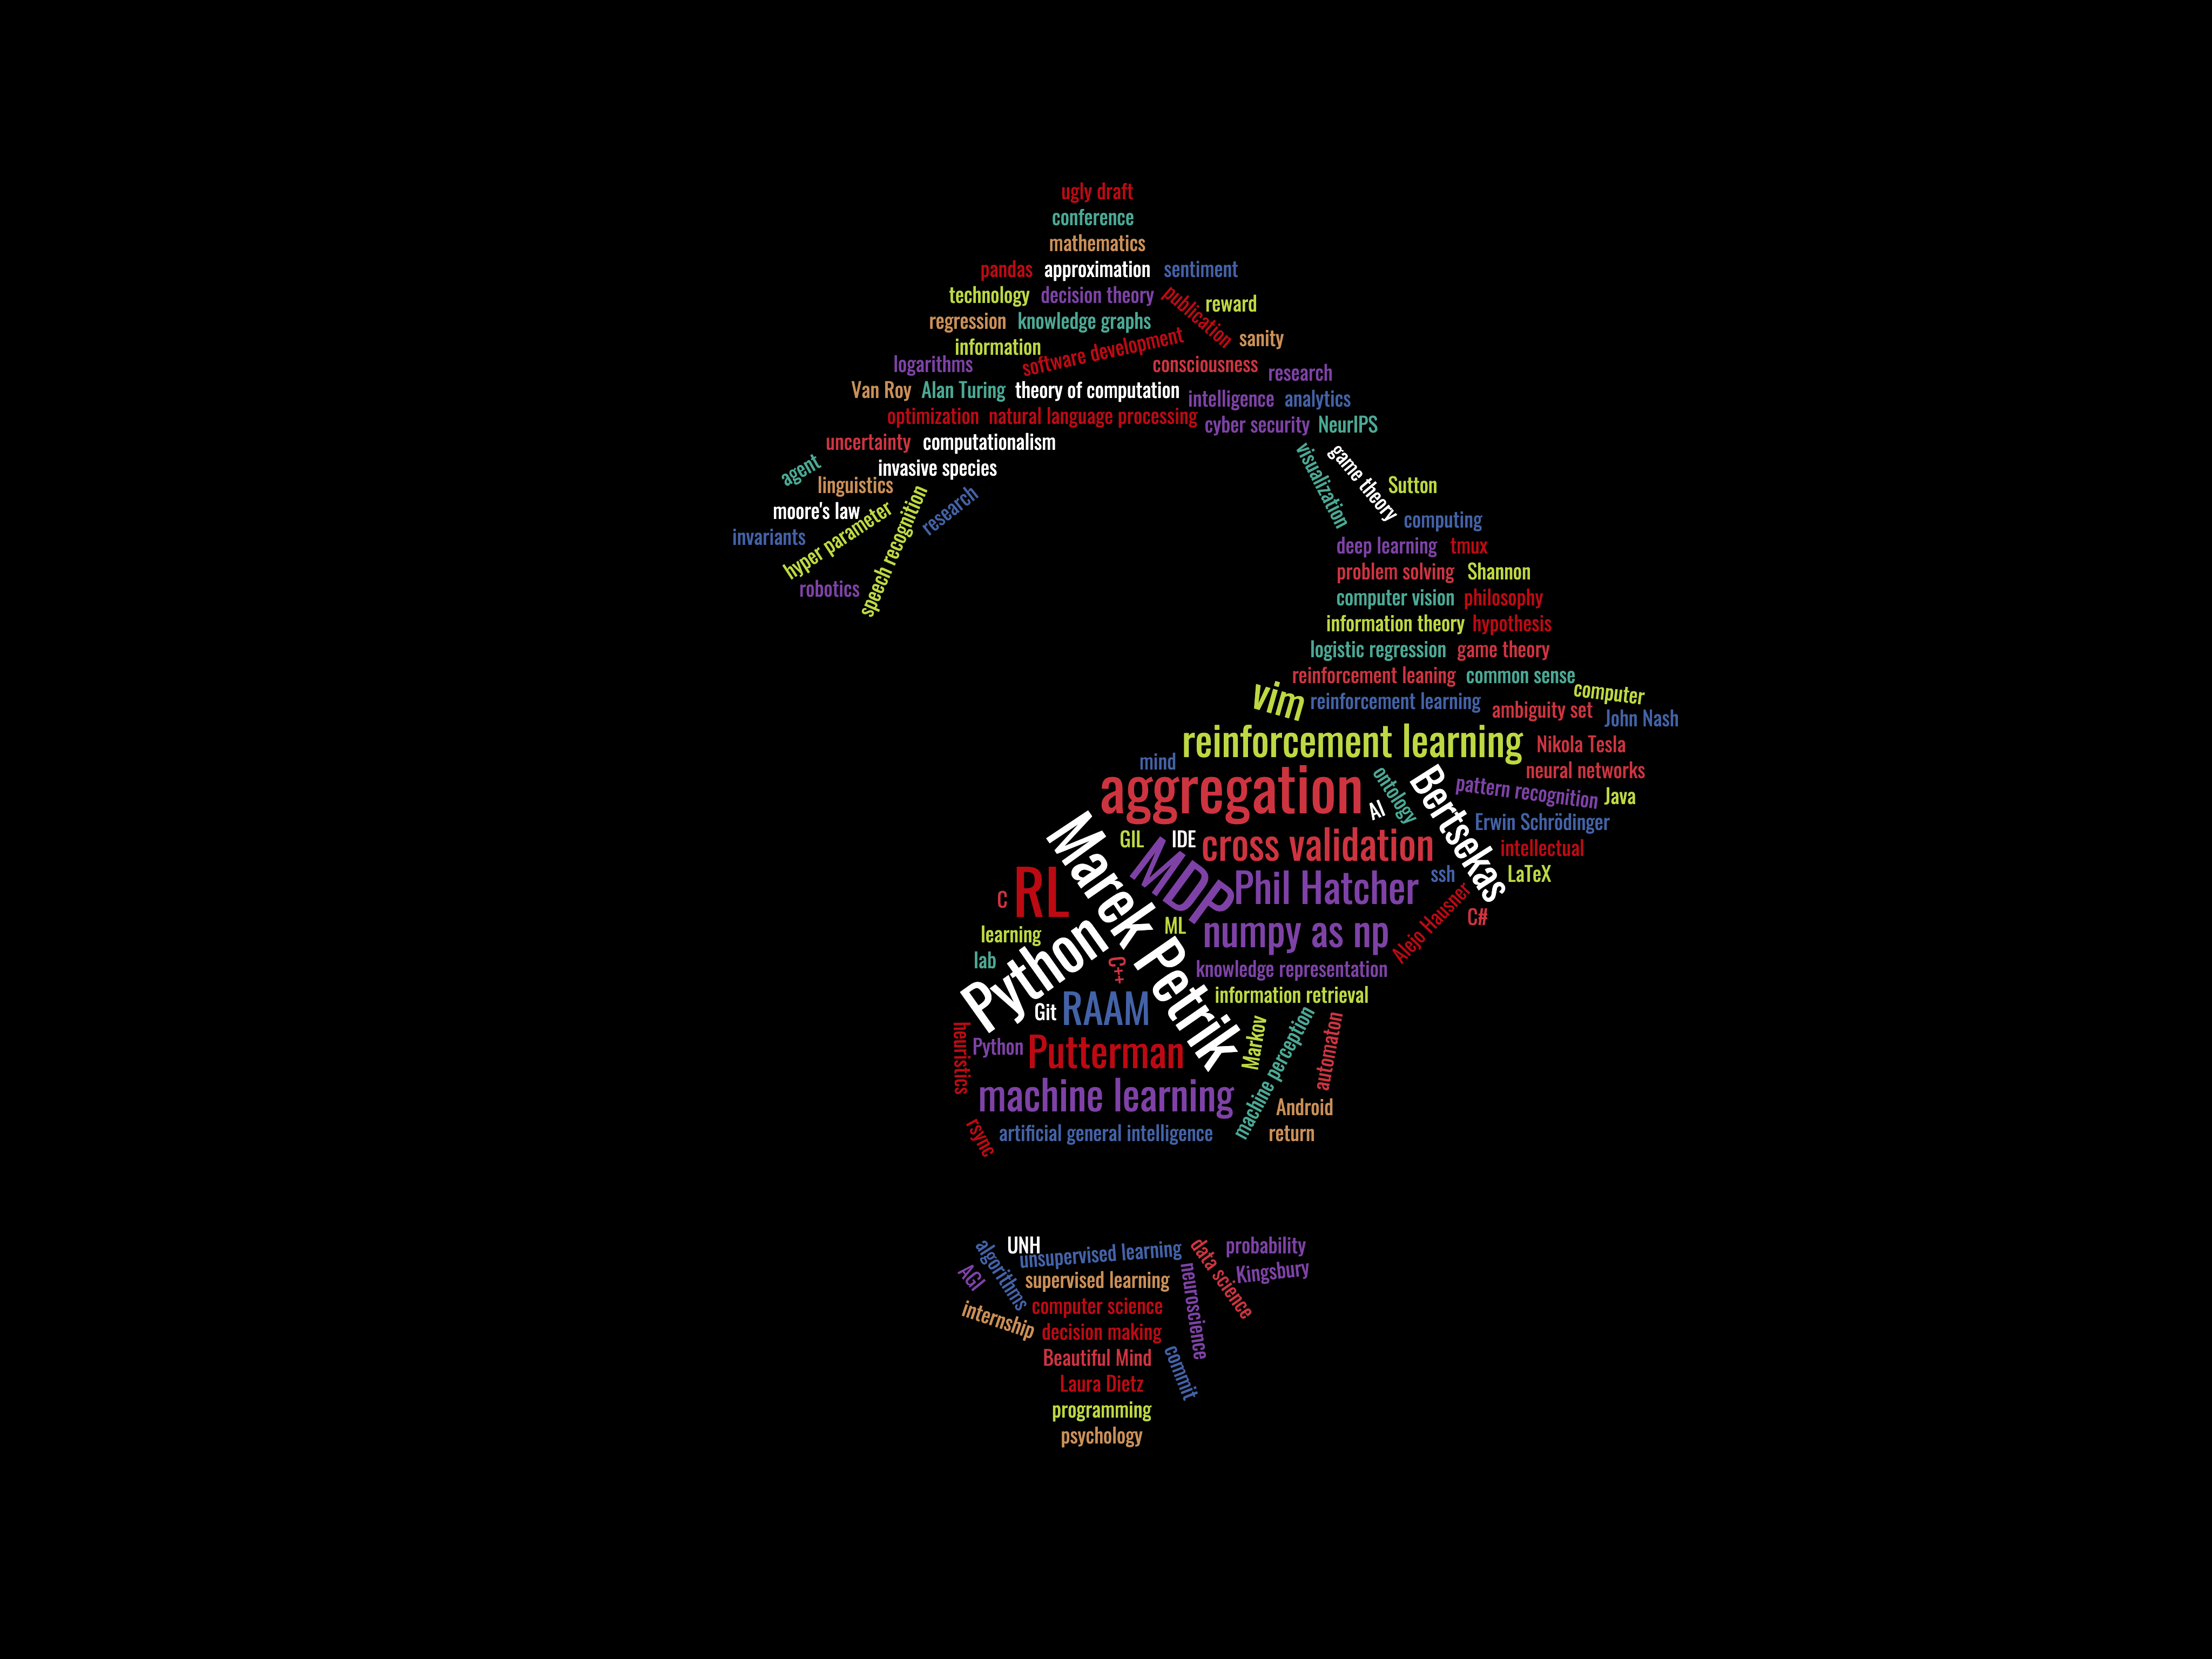
\includegraphics[width=1\columnwidth]{wordcloud.png}
    
\end{frame}

\begin{frame}
    \frametitle{Outline}

    \begin{itemize}
        \item Problem
        \item Examples
        \item Motivation
        \item Outline
        \item BODY
        \item Q&A
    \end{itemize}
\end{frame}


\begin{frame}
    \frametitle{State Aggregation}
    \label{fm:sta}
    \framesubtitle{Problem}
    
    \begin{itemize}
        \item Problem \textit{approximation} 
        \item based on \textit{aggregation}.
        \item in value space
        \item feature-based parametric approximation
    \end{itemize}
 
\end{frame}




\begin{frame}
    \frametitle{Why State Aggregation?}
    \framesubtitle{Problem}

    \begin{itemize}
        \item less computational power
        \item more tractable problem
        \item analytically transparent approximation
            \begin{itemize}
                \item compared to Neural Networks
            \end{itemize}
    \end{itemize}
    
    
\end{frame}


\begin{frame}
    \frametitle{Aggregate State}
    \framesubtitle{Problem}

    \begin{itemize}
        \item special group of multiple [original] states
        \item 
    \end{itemize}
    
\end{frame}

\begin{frame}
    \frametitle{Nomenclature}
    \framesubtitle{Problem}

    
    \begin{itemize}
        \item Original State
            \begin{itemize}
                \item 
            \end{itemize}
        \item Aggregate State
    \end{itemize}

\end{frame}


\begin{frame}
    \frametitle{Idea}
    
    
\end{frame}


\begin{frame}
    \frametitle{How Many Bins?}
    \framesubtitle{Idea}

    Number of buckets to split original states into:
    \begin{itemize}
        \item range split aggregation
    \end{itemize}
    
    
\end{frame}


\begin{frame}
    \frametitle{}
    
    
\end{frame}

\begin{frame}
    \frametitle{}
    
    
\end{frame}

\begin{frame}
    \frametitle{}
    
    
\end{frame}

\begin{frame}
    \frametitle{}
    
    
\end{frame}

\begin{frame}
    \frametitle{}
    
    
\end{frame}

\begin{frame}
    \frametitle{}
    
    
\end{frame}

    

\end{document}